\documentclass[twocolumn]{aastex61}
\usepackage{natbib}
\bibliographystyle{apj}
\usepackage{graphicx}
\usepackage{amsmath}

\newcommand{\citeth}[1]{(\citeauthor{#1}\ \citeyear{#1})}
\newcommand{\citethnop}[1]{\citeauthor{#1}\ \citeyear{#1}}
\newcommand{\citethnopp}[1]{\citeauthor{#1}\ (\citeyear{#1})}

\def \lya {Ly$\alpha$ }
\def \mkms {{\rm \; km\;s^{-1}}}
\def \msunperyr {{\; M_{\odot}\rm \;yr^{-1}}}

\begin{document}
\title{A VLT/FORS2 Narrowband Imaging Search for \ion{Mg}{2} Emission Around $\lowercase{z}\sim0.7$ Galaxies }
\author{Ryan Rickards Vaught}
\affiliation{San Diego State University 5500 Campanile Dr, San Diego, CA 92182}
\affiliation{Department of Physics, University of California, San Diego, CA} 
 
 \author{Kate H. R. Rubin }
 \affiliation{San Diego State University 5500 Campanile Dr, San Diego, CA 92182}
 
 \author{Fabrizio Arrigoni Battaia }
 \affiliation{Max-Planck-Institut fur Astronomie, Konigstuhl 17, D- 69117 Heidelberg, Germany}

 \author{J. Xavier Prochaska}
 \affiliation{Astronomy \& Astrophysics, UC Santa Cruz, 1156 High St., Santa Cruz, CA 95064 USA}
 
\author{Joseph Hennawi,}
\affiliation{Department of Physics, Broida Hall, University of California, Santa Barbara, CA 93106-9530}

\correspondingauthor{Ryan Rickards Vaught}
\email{rjvaught@gmail.com}

\begin{abstract}

Galactic-scale outflows are thought to be the primary mechanism in the removal of cool gas from star-forming galaxies. Presently, the mass and energy of these flows remain poorly constrained. One way to better constrain these parameters is to measure the spatial extent of the outflow; however, measuring this quantity via spectral methods has been traditionally very difficult due to the faintness of emission lines tracing outflowing material. We perform a VLT/FORS2 narrowband imaging of 5 star-forming galaxies at redshift $z=0.67-0.69$ in the GOODS-S field as part of an effort to spatially resolve and constrain the radial extent of large-scale outflows traced by \ion{Mg}{2} emission. These observations probe \ion{Mg}{2} to unmatched surface brightness limits of 5.74 $\times$ $10^{-19}$ ergs sec $^{-1}$ cm$^{-2}$ arcsec$^2$ (5$\sigma$). We do not detect any extended \ion{Mg}{2} emission in any of our galaxies, suggesting that the wind material does not extend beyond the galaxies' stellar component. Our observations also allow us to create the first ever spatially-resolved map of  \ion{Mg}{2} absorption, revealing approximately constant absorption strengths across the galaxy disks.

\end{abstract}

\keywords{Galaxy Evolution, Galactic Winds}

\section{Introduction}\label{sec:intro}
Galactic winds play a critical role in regulating the star formation rates and stellar masses of galaxies \citeth{Werk_2014}; however, the physical mechanism that powers these galactic winds remains uncertain. Some possible mechanics have been proposed by theoretical studies that include thermal pressure from core collapse supernova, radiation pressure from starbursts and finally cosmic ray pressure (\citethnop{Larson_1974}; \citethnop{Chevalier_1985}; \citethnop{Springel_2003}; \citethnop{Sugahara_2017}). However it is very difficult to distinguish between these mechanisms with current observational techniques. Additionally, the impact galactic winds have on their host galaxies (i.e, their mass and energy content) has remained difficult to constrain with observations.

An accurate picture of what types of galaxies host outflows comes from numerous absorption line studies of galaxies (\citethnop{Veilleux2005}; \citethnop{Weiner2009}; \citethnop{Martin2012}; \citethnop{Rubin_2014}). Outflows are detected by measuring the blueshift (outflow) or redshift (inflow) of absorption transitions with respect to the host galaxy systematic velocities. Spectroscopy of galaxies from low to high redshifts probing cold gas which absorbs in \ion{Na}{1} and cool gas in \ion{Mg}{2} has revealed outflows in most galaxies that host active star-formation (e.g. \citethnop{Martin2012}; \citethnop{Rubin_2014}). Even though these probes can ascertain: the radial velocity, column density and covering fraction of the flow, this method is weak in constraining the overall radial extent and provides no information on the morphology of the outflow.

One novel way of developing these constraints is to trace the extent of winds in emission. This has been demonstrated in the optical using rest frame near infrared transitions (i.e H$\alpha$ and \ion{O}{3} etc) as tracers for nearby starbursts (\citethnop{Matsubayashi2009}; \citethnop{Veilleux2009}; \citethnop{Tripp2011}) because these transitions can trace the warm shock heated phase of the gas. However, it is difficult to use these rest frame near infrared transitions to probe winds at higher redshift because the faint emission can be redshifted into the infrared where the sky background is bright. At higher redshifts, it is advantageous to trace winds in the optical with the rest frame ultraviolet ion, \ion{Mg}{2} (Weiner et al. 2009; Kornei et al. 2013)\nocite{Weiner2009, Kornei2013}

Typically, studies of winds using \ion{Mg}{2} have focused on its absorption kinematics. However, recently in a study by \cite{Rubin_2011}, strong \ion{Mg}{2} emission with a P-Cygni line profile was observed in the 2D spectrum of a strongly star-forming galaxy at redshift $z = 0.694$.  This emission was the first detection of an outflow beyond the spatial extent of the galaxy continuum in the distant universe, with a minimum spatial extent  $>$ 7 kpc. One proposed production mechanism for the galaxy's observed \ion{Mg}{2} line profile is photon scattering. 

In this mechanism, \ion{Mg}{2} ions in the region of the wind closest to the observer will absorb continuum photons in the resonant transitions, $\lambda_{2796}$ and $\lambda_{2803}$. Once these transitions are excited, they may only decay back to the ground state and if the optical depth of the gas is high, then the gas will resonantly trap the absorbed photons. Because the photons are absorbed in the rest frame of the gas, the absorption will be blueshifted relative to the galaxy's systematic velocity. The \ion{Mg}{2} ions in the section of the wind farthest from the observer will absorb and scatter photons that are redshifted relative to the front portion of the wind. Because the photons are redshifted, the photons will be able to travel freely towards the observer through the wind to produce emission at and redward of the systematic velocity of the galaxy \citeth{Rubin_2011}. The photon scattering model, as explained, is described for the geometry of an isotropic wind \citeth{Prochaska_2011}. For anisotropic bi-conical winds, the emission induced from photon scattering will be highly suppressed. Since the first detection of \ion{Mg}{2} emission by \citeth{Rubin_2011}, further detections of extended \ion{Mg}{2} emission are by \cite{Erb2012} and \cite{Martin2013} have shown that emission is stronger for higher mass galaxies and that outflows can extend out to at least 18 kpc.

We aim to take advantage of this photon scattering as we present the first narrowband imaging of \ion{Mg}{2} line emission of 5 star-forming ($z \sim 0.7$) galaxies located in the deep Great Observatories Origins Deep Survey south (GOODS-S) field. The value in using narrowband imaging is the ability to spatially resolve any absoroption and emission from a galaxy. We use two filters: a line filter and a continuum filter. The line filter covers the \ion{Mg}{2} doublet, while the continuum filter is off-set from line filter. The continuum filter will allow us to observe the continuum level of the galaxy near the \ion{Mg}{2} doublet. With the resulting images taken using the two filters, we can subtract the continuum image from the \ion{Mg}{2} image, effectively creating an image that contains only photons from \ion{Mg}{2}. Contrary to 1D spectra, the narrowband imaging has the ability to measure the surface brightness, optical depth and radial extent of a wind. This narrowband imaging will allow us to create the first ever spatially resolved map of \ion{Mg}{2} emission.


\section{Observations and Data Reduction}

\subsection{Sample Selection}
Our target galaxies were selected from a Keck/LRIS survey of UV absorption lines in $\approx 100$ objects having redshifts $0.3< z < 1.4$ and $B_{AB}< 23$ in fields with deep \emph{HST}/ACS imaging (Rubin et al. 2014)\nocite{Rubin_2014}.  In particular, this parent survey targeted galaxies in a total of nine Keck/LRIS pointings located in both of the GOODS fields (\citeauthor{Giavalisco2004} \citeyear{Giavalisco2004})and the AEGIS survey field (the Extended Groth Strip; Davis et al. 2007)\nocite{Davis2007}.  In inspecting the redshift distribution of the portion of this sample observable from the Southern Hemisphere, we uncovered a narrow peak of nine galaxies in the interval $0.66 < z < 0.68$.  This peak is in fact the global maximum of the distribution, as all other bins of width $\Delta z = 0.02$ have at most four galaxies.  Moreover, there are two narrow interference filters available on VLT/FORS2 centered at $\lambda \sim 468.4$ and 472.6 nm which cover the \ion{Mg}{2} $\lambda \lambda 2796, 2803$ transition in precisely this redshift interval.  We selected our final sample of five of these galaxies at $0.66 < z < 0.68$ to be close on the sky such that they could be imaged in a single $7' \times 7' $ FORS2 pointing.  

The absorption line modeling presented in (Rubin et al. 2014)\nocite{Rubin_2014} indicates that these five galaxies are driving strong outflows traced by \ion{Mg}{2}  with velocities $\sim150-420\mkms$ and equivalent widths (EW) $\sim 2-3$ \AA.  Modeling of the galaxy broad-band spectral energy distributions obtained from multi-wavelength ancillary imaging data yields star formation rates (SFR) ranging from $\sim4$ to $40\msunperyr$ and stellar masses in the range $\log M_*/M_{\odot}\sim 9.9-11.0$. The properties of the sample, as well as precise target coordinates, taken from \cite{Rubin_2014} are listed in Table \ref{tab:prop}. 


\subsection{VLT/FORS2 Observations}
The data were taken in service-mode using the FORS2 instrument on the VLT 8.2m telescope Antu between October 2012 and February 2013. 
We used two narrowband filters, HeII+47 and HeII/3000+48, that have peak transmission at wavelengths that correspond to the \ion{Mg}{2} doublet lines at our sample redshift of $z\approx 0.7$ (see Table \ref{tab:filters}). The transmission curves are plotted along with each galaxy's spectrum in Figure~\ref{fig:spec_images}.

FORS2 has a pixel scale of $0.25''$ pixel$^{-1}$ and a field of view of $7'\times7'$. Summing the individual exposure times for each image results in a combined exposure time of $10.0$ hours each for the HeII+47 and HeII/3000+48 filters. Our observations were carried out under photometric and thin cloud conditions (program ID: 090.A-0427A). The seeing (see Figure \ref{fig.seeing}) ranged from 0.5 arcsec to 2.5 arcsec. The data were taken with three pointings offset by 0.25'.

\begin{figure*}[!ht]
\centering
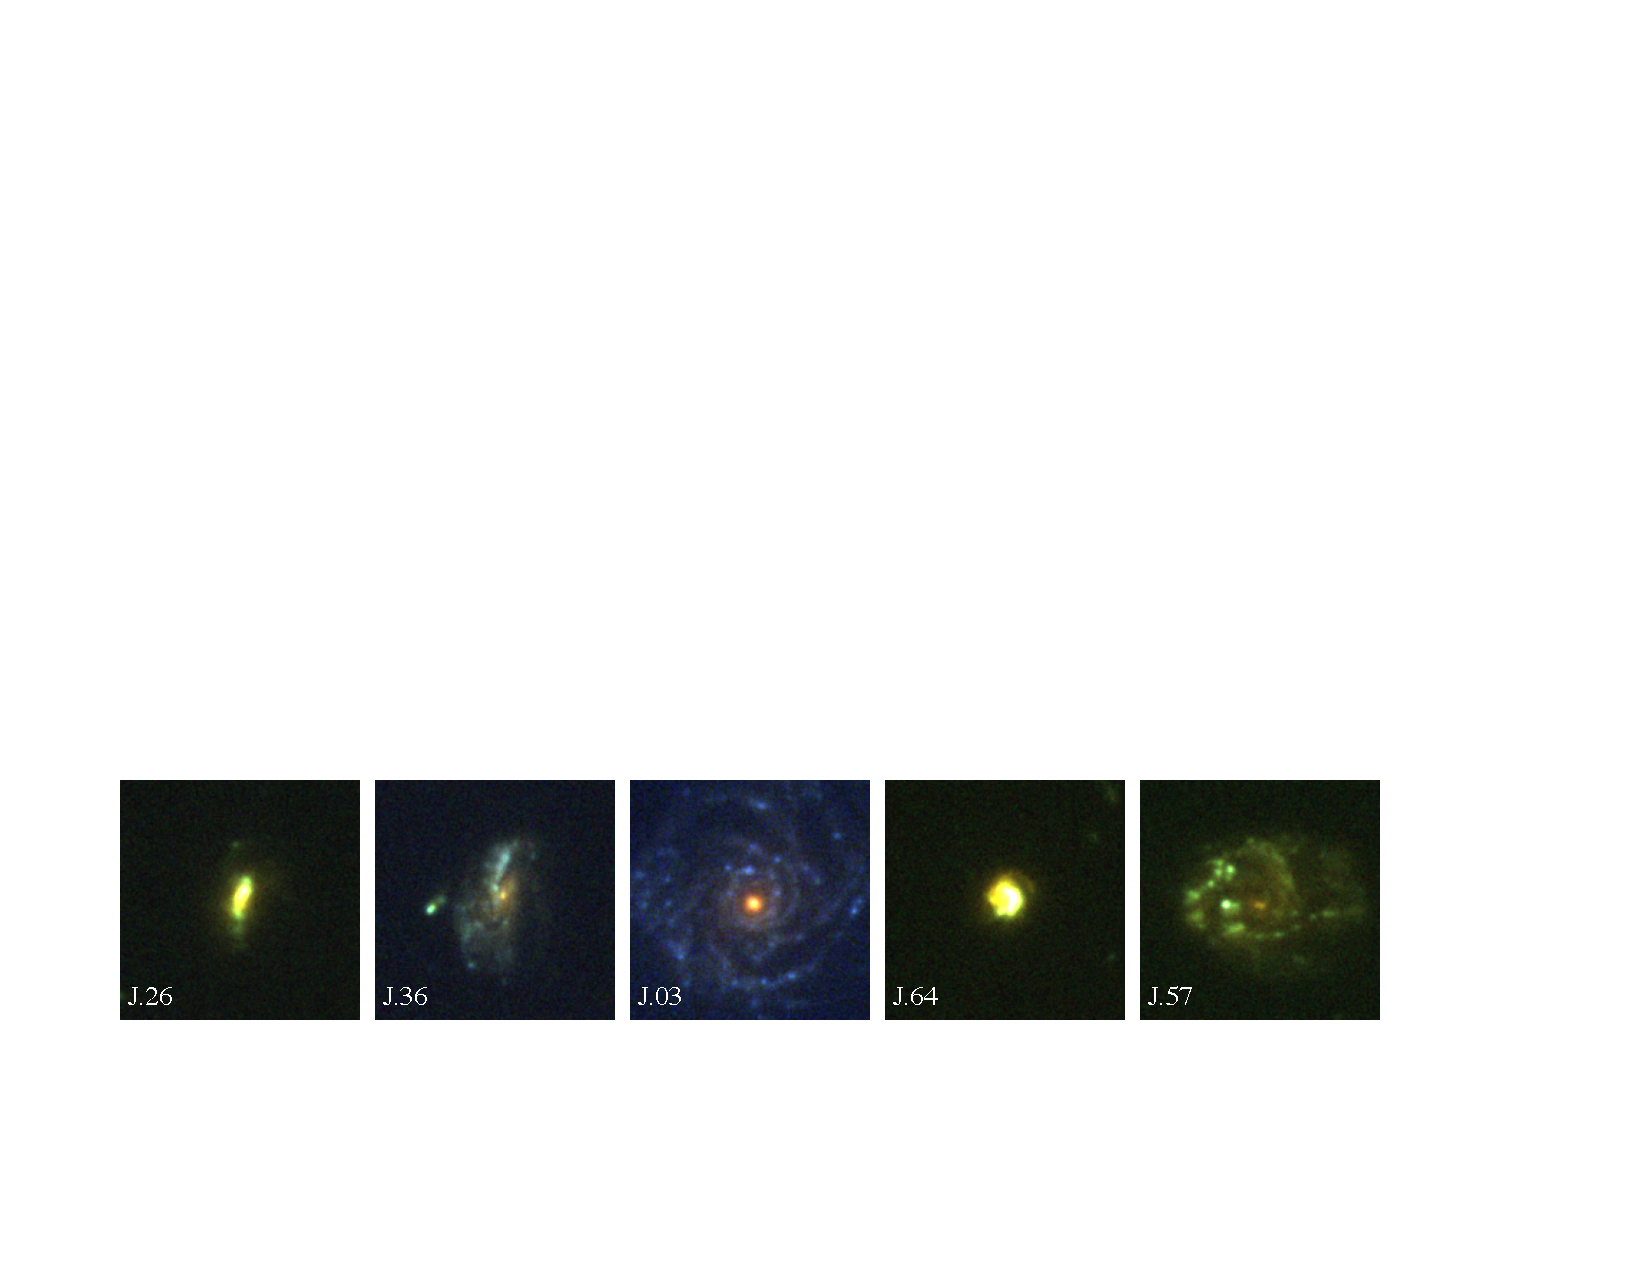
\includegraphics[scale=.73]{../Figures/fors2_color_imstamps.pdf}
\caption{Color imaging of our sample galaxies in the \emph{HST}/ACS F435W, F606W, and F775W filters obtained as part of the GOODS survey (\citeauthor{Giavalisco2004} \citeyear{Giavalisco2004}). Each image is 5'' $\times$ 5''.\label{fig:hstims}}
\end{figure*}

\begin{figure*}[!htb]
\centering
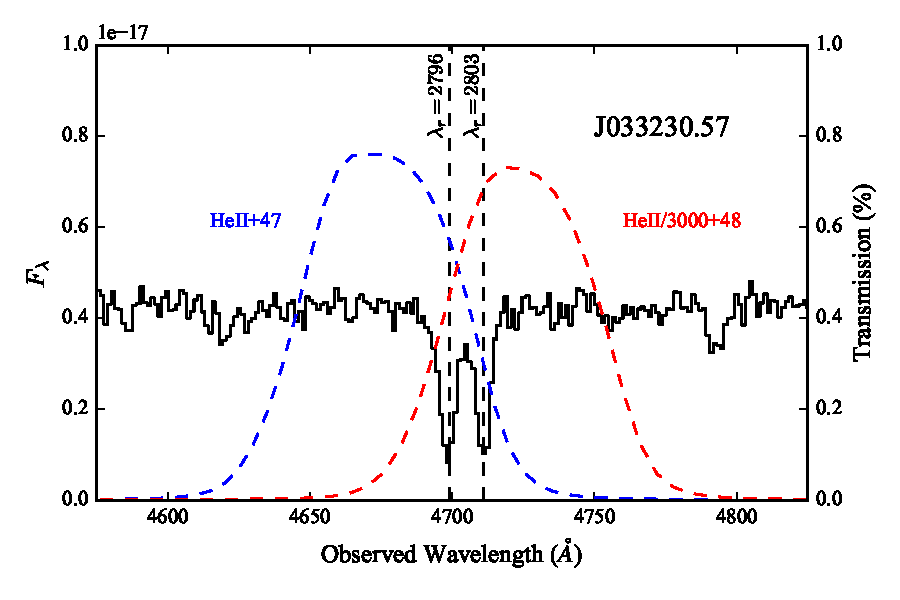
\includegraphics[scale=0.58]{../Figures/filt_57_spectra.pdf}
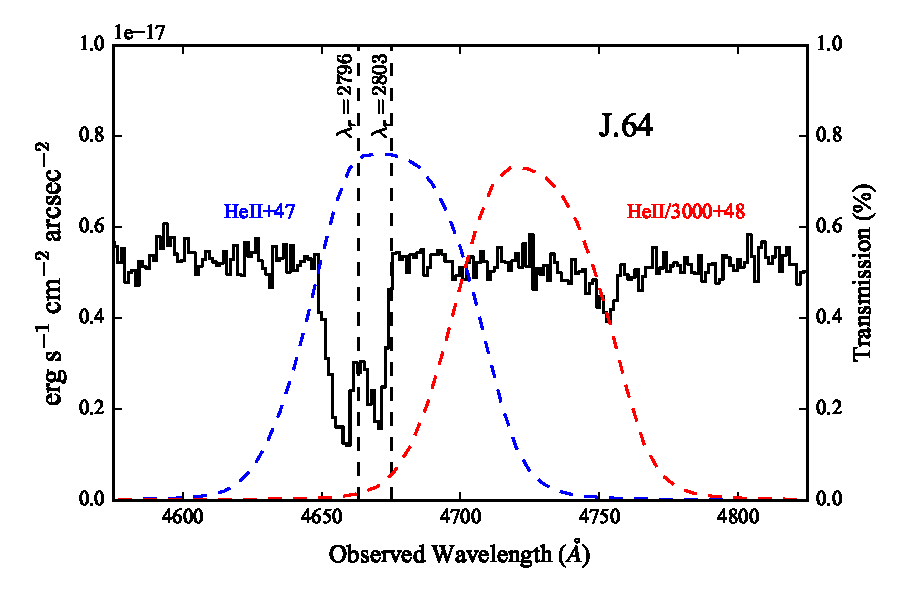
\includegraphics[scale=0.58]{../Figures/filt_64_spectra.pdf}
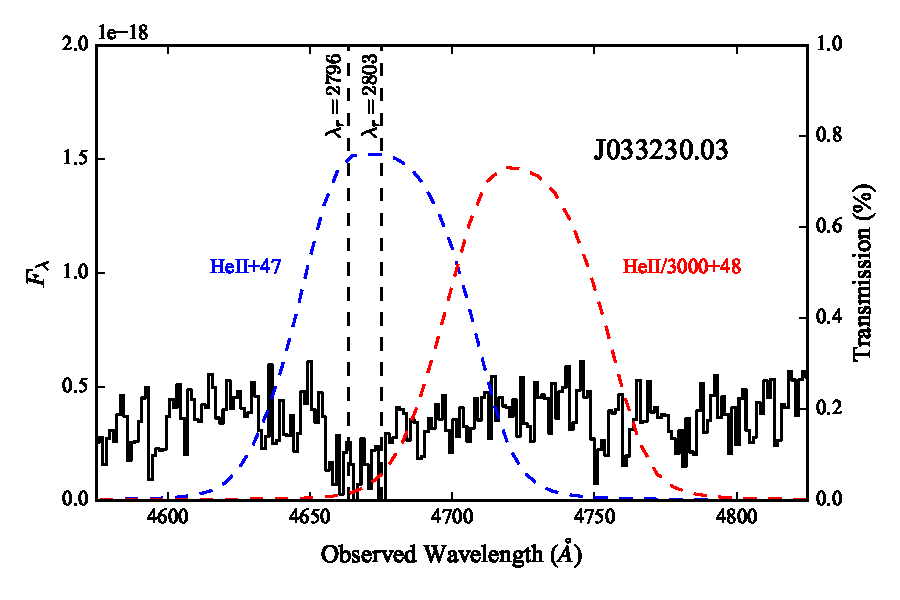
\includegraphics[scale=0.58]{../Figures/filt_03_spectra.pdf}
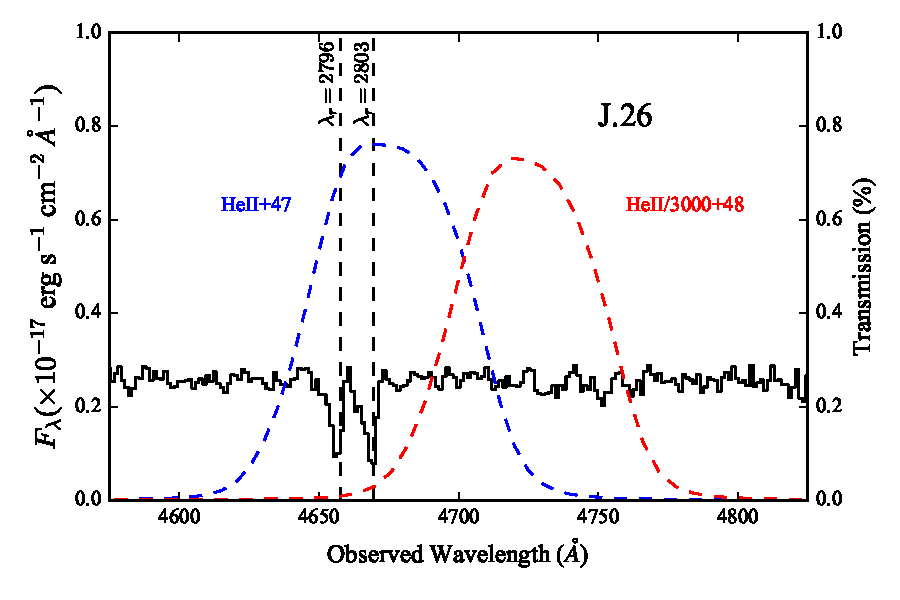
\includegraphics[scale=0.58]{../Figures/filt_26_spectra.pdf}
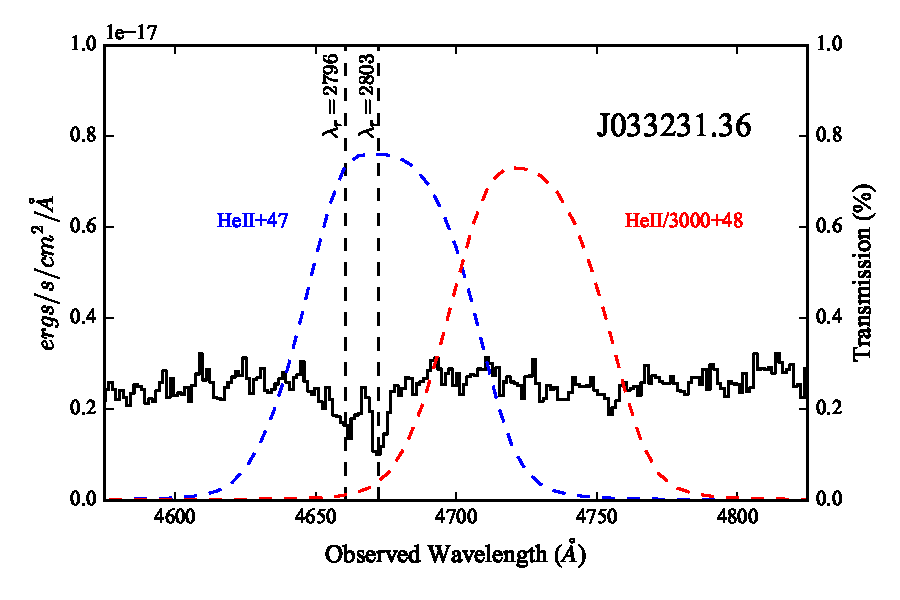
\includegraphics[scale=0.58]{../Figures/filt_36_spectra.pdf}
\caption{KECK/LRIS spectrum of the sample galaxies and the transmission curves of the filters HeII+47 and HeII/3000+48. The left-hand axis is in units of flux density and the right-hand axis is the percentage of light transmitted the filter at each wavelength. Vertical dotted lines indicate the wavelength of the redshifted \ion{Mg}{2}\ doublet. The \ion{Mg}{2}\ doublet falls fortuitously at the central wavelength of the HEII+47 filter.}
\label{fig:spec_images}
\end{figure*}

\begin{figure}[h]
\centering
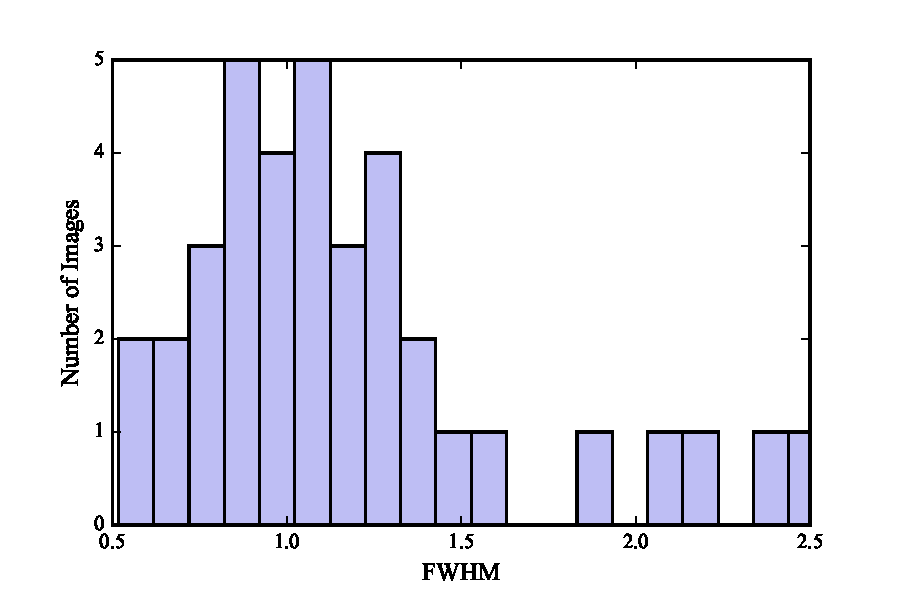
\includegraphics[scale=.55]{../Figures/avg_seeing_HEII.pdf}
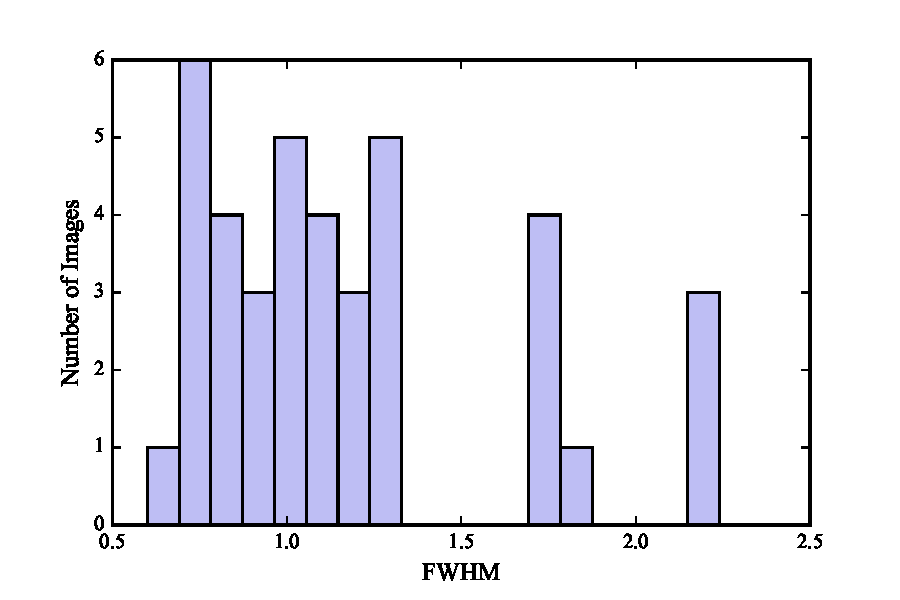
\includegraphics[scale=.55]{../Figures/avg_seeing_HEII3000.pdf}
\caption{  Distribution of seeing conditions for individual exposures comprising our dataset.
\textbf{Top}: Seeing distribution for the 38 HeII+47 images. The median seeing in this filter is $1.03\arcsec$.
\textbf{Bottom}: Same distribution for the 38 HEII/3000+48 images. The median seeing is $1.08\arcsec$. 
The seeing conditions were calculated by ESO and were provided in the header of each science image.
\label{fig.seeing}}
\end{figure}



\subsection{Supplemental Keck/LRIS spectra}
In addition to VLT imaging, in the present analysis we utilize galaxy spectra taken from the \cite{Rubin_2014} Keck I Low Resolution Imaging Spectrometer (LRIS) program. A $0.9''$ slit width was used for all slitmasks and the median FWHM resolution for the spectra is 274 km s$^{-1}$ at $\lambda_{\rm rest} \approx$ 2800 \AA\ and $286\mkms$  at $\lambda_{\rm rest}\approx$ 2600 \AA\ (see Figure \ref{fig:spec_images}).

\subsection{Image Reduction}
The data were reduced using custom routines written in \textbf{Python}. 
The images were first corrected by subtracting and removing the overscan region of the CCD. 
Then the images were bias-subtracted and flat-fielded using twilight flats.
To improve the flat-fielding essential for detecting faint extended emission across the fields,we further correct for the illumination patterns using night-sky flats. The night-sky flats were produced by combining the unregistered science frames with an average sigma-clipping algorithm after masking out all the objects, and any bad pixels. Each individual image was cleaned of cosmic rays and bad pixels by utilizing the L.A. Cosmic algorithm.
The astrometry solutions were calculated via Astrometry.net (Lang et al. 2010)\nocite{Lang} with a standard deviation in the galaxy coordinates of $\sigma \approx 0.10''$. Before image stacking, we ran each frame through \textbf{SExtractor} \citeth{Bertin} in order to create a root mean square (RMS) map of each science image.
These frames, in addition to the science images, are stacked to create a co-added RMS image.

The final stacked images for each filter is obtained using \textbf{SWarp} \citeth{Bertin}.
Each individual frame is first sky-subtracted using a background mesh size of 256 pixels which is approximately $64''$. 
We chose the mesh size to be large enough such that the extended emission is not mistakenly subtracted (Arrigoni Battaia et al. 2015) \nocite{Battaia_2015}. 
The frame, after background-subtraction, is resampled onto a common astrometric solution using a \textit{Lancosz3} interpolation kernel. 
The images are average-combined and weighted by the night-flat image in order to increase the signal-to-noise of any \ion{Mg}{2} emission. \textbf{SWarp} is also configured to produce RMS weight maps from our \textbf{SExtractor} weighted images. Our final stacked images in each filter are shown in Figure~\ref{fig:stacked_image} with the target galaxies indicated.  

One side effect from stacking is that the east and west borders of each image contain greater noise compared to the center of the image. This is due to the imperfect overlap of the 3 pointings used. However, the sample galaxies are sufficiently distant from these low S/N regions that their photometry is not affected.


\begin{table}[h!]
\caption{VLT/FORS2 Observations: Filter and exposure properties of the VLT observations. The width of the transmission curves are calculated by convolving the transmission curve with the total wavelength range of the filter. These values differ slightly from those reported by the European Space Observatory. }
\begin{tabular}{llllll} \hline \hline 
Filter & $\lambda_{eff}$(\AA)\footnote{$\lambda_{eff}$ is the effective wavelength of the filter transmission curve.} & $\lambda_{width}$(\text{\AA})    & $N_{\text{img}}$   & $t_{tot}(s)$ & $S$\footnote{S is in units of $10^{-17}$ ergs counts$^{-1}$ cm$^{-2}$ }\smallskip  \\ \hline 
HeII  & 4675.21 & 50.11 & 38  & 35,959 & 2.45 \\
HeII/3000 & 4722.46  & 44.82 & 38 &   36,937 & 2.40       \\ \hline
\end{tabular}
\label{tab:filters}
\end{table}

\begin{table*}[t]
\centering
\caption{Properties of 5 galaxies in our sample :  All galaxies are at roughly the same redshift. The star formation rates for the sample range from 3.8 to 40.5 solar mass per year. The EW include both components of the \ion{Mg}{2} doublet and were calculated with Eq. \ref{eq:specEW} and the supplemental Keck/LRIS spectra. \emph{HST}/ACS images of the galaxy sample are shown in Figure~\ref{fig:hstims}. The Keck/LRIS spectroscopy of this sample published in \cite{Rubin_2014} is shown in Figure~\ref{fig:spec_images}}
\begin{tabular}{lllllll} \hline \hline
Object & R.A. & Dec  & $z$ & SFR($M_{\odot}$ yr$^{-1}$) & $\log{M_{*}/M_{\odot}}$ & EW(\AA) \smallskip      \\ \hline 
J033225.26-      & 03:32:25.26 & -27:45:23.9 & 0.6660 & $9.1_{-3.7}^{+1.3}$& $9.86_{-0.04}^{+0.05}$ & $7.539\pm 0.354$\\ 
274524.0     & &  &  &         \\
J033231.36-      & 03:32:31.35 & -27:47:24.9 &   0.6669 & $10.5_{-1.6}^{+1.7}$ & $10.02_{-0.03}^{+0.03}$&$5.835 \pm 0.493$\\
274725.0      & &  &   &        \\
J033230.03-      & 03:32:30.03 & -27:43:47.2  &   0.6679 & $3.8_{-0}^{+0}$ & $10.98_{-0.0}^{+0.01}$ &$12.794 \pm 1.710$\\
274347.3      & &  &   &        \\
J033229.64-      & 03:32:29.64 & -27:42:42.5 & 0.6671 & $40.5_{-12.1}^{+8.2}$ & $10.30_{-0.03}^{+0.07}$ &$13.239 \pm 0.263$\\
274242.6     & &  &     &      \\
J033230.57-      & 03:32:30.56 & -27:45:18.2 &   0.6807  & $12.6_{-2.1}^{+1.7}$ & $10.48_{-0.07}^{+0.03}$ &$6.106 \pm 0.370$ \\
274518.2      & &  &  &         \\ \hline 
\end{tabular}
\label{tab:prop}
\end{table*}


\subsection{Absolute Flux Calibration}
We acquired observations of the standard star GD50 from archival ESO calibration imaging at 4 independent epochs.From this standard we calculated the atmospheric extinction coefficients to be 0.181 magnitudes for the HeII/3000+48 filter and 0.190 magnitudes for the HeII+47 filter. Since we have imaging of the standard star GD50 in our two filters, and access to GD50's spectral energy distribution (cite!) and each filter's transmission curve through the ESO website, we are able to perform absolute flux calibration using the methods of Jacoby et al. (1990). We first convolve the spectral energy distribution of the standard star, $F(\lambda)$ in ergs sec$^{-1}$ \AA$^{-1}$ cm$^{-2}$, with that of the known transmission curve of the filter, $T_{i}(\lambda)$. This yields $F_i$, the total observable flux in each bandpass filter $i$ with units of ergs sec$^{-1}$ cm$^{-2}$:
\begin{equation*}
F_{i}=\int F(\lambda)T_{i}(\lambda)d\lambda.
\end{equation*}
It is not uncommon to assume that $F(\lambda)$ is constant over the small width of the filter. However, our filter transmission curves are sampled at $5$\ \AA\ intervals which is the same sampling as the spectral energy distribution of the standard star obtained from the ESO archives. Therefore we calculate the integral numerically.
The system sensitivity, including the defects of the telescope optics and detector response is then given by
\begin{equation*}
S_{i}=\dfrac{F_{i}}{C10^{k_{i}A}},
\end{equation*}\\
where $k_i$ is the extinction in magnitudes per airmass, A is the airmass for each individual exposure, C is the measured count rate of the standard star and $S$ is in units of ergs counts$^{-1}$ cm$^{-2}$. Before image co-addition, each science image is corrected for atmospheric extinction by multiplying each frame by $10^{k_{i}A}$. Next, the image is divided by the exposure time, effectively putting the image in units of counts per sec. After co-addition, the images are then multiplied by the appropriate sensitivity factor $S_{i}$. This puts the final images in the appropriate flux units ergs sec $^{-1}$ cm$^{-2}$.

\begin{figure*}[ht!]
\centering
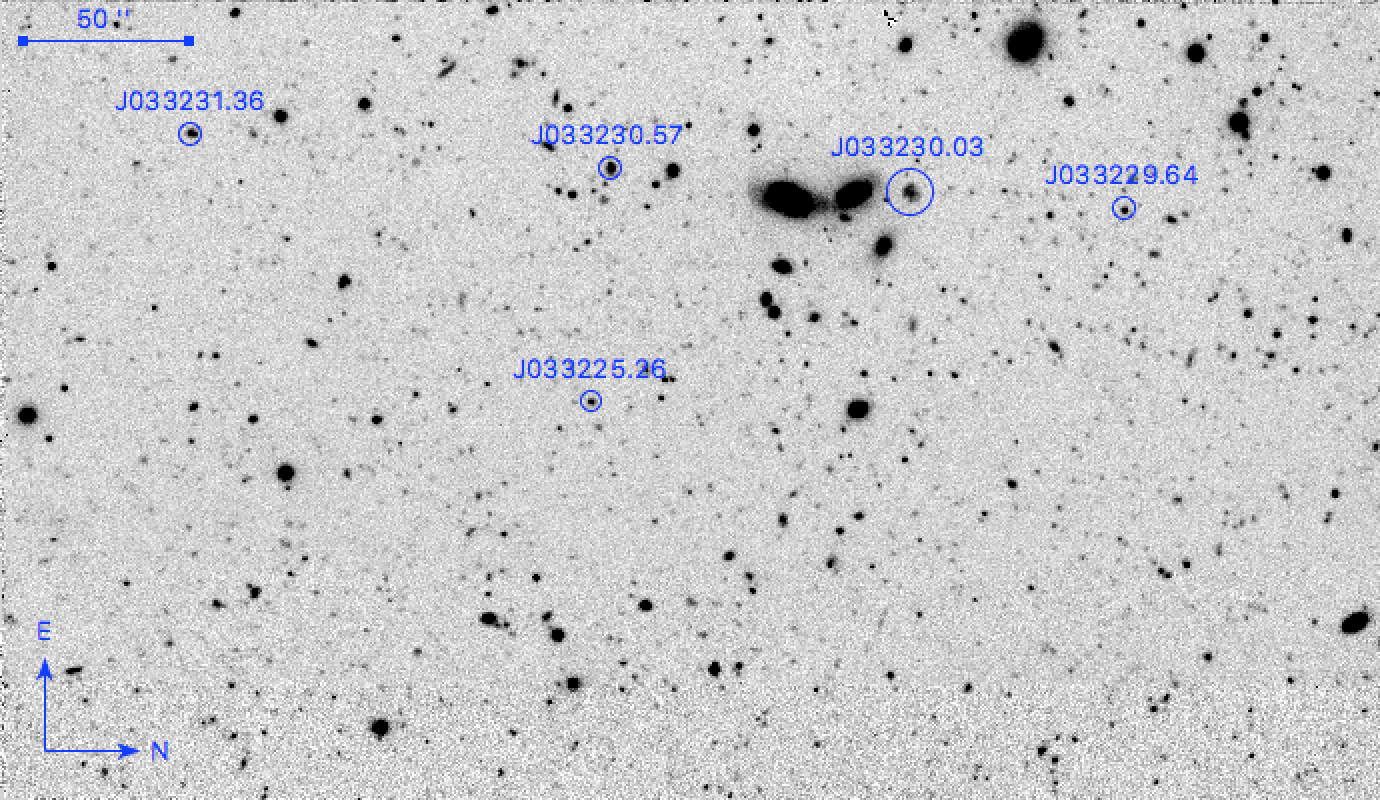
\includegraphics[scale=.61]{../Figures/HEII_final.png}
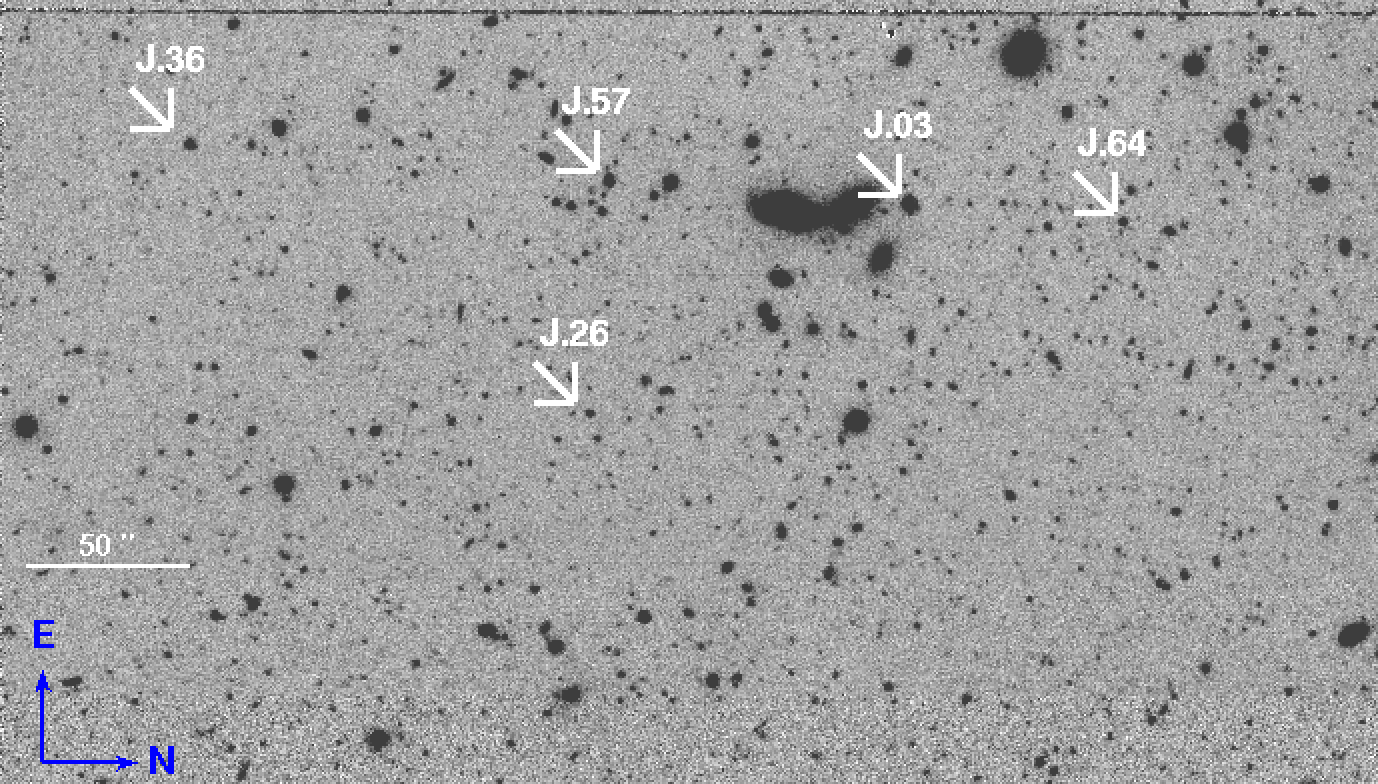
\includegraphics[scale=.61]{../Figures/HEII3000_final.png}
\caption{Top: HeII+47 image after stacking. Bottom: HeII3000+48 image after stacking. The exposure time of each image is $\approx 10$ hours. Each image has a FOV of $7' \times 7'$ which fortuitously contains the full sample of galaxies (indicated by the blue circles) in a single pointing. East is up and North is right.
\label{fig:stacked_image}}
\end{figure*}

\section{Analysis}
We have two goals for our study: (1) assess the surface brightness of line emission in the \ion{Mg}{2} transition in and around each target galaxy; and (2) spatially resolve the morphology of the strong \ion{Mg}{2} absorption observed against the galaxy continua.  To reach the both of these goals, we must perform accurate subtraction of the continuum flux of each object from the filter covering the targeted line emission. For four of the five objects in our sample, the HeII+47 image includes both line and continuum emission, and the HeII3000+48 image provides a high S/N measurement of the continuum only $\approx30$ \AA\ redward of the line emission in the rest-frame.  We detail our method of continuum subtraction using these data in Section~\ref{sec.cont_sub} below, and follow with a presentation of the resulting surface brightness profiles (Section~\ref{sec.sb}) and EW images (Section~\ref{subsec.ew}).


\subsection{Spectral Correction}
With the supplementary spectra from \citeth{Rubin_2014}, we can fit the continuum and determine the slope of each galaxy spectrum in order to test whether the spectral slope gives rise to differences in continuum flux between the two filters. We use the interactive fitting routine \textbf{lt\_continuumfit} from the linetools package (Prochaska et al. 2016)\footnote{https://github.com/linetools/linetools}\nocite{Prochaska2016} to fit the continuum. By fitting the continuum we are masking the absorption features and making an effectively flat spectrum, which we use as a model. We find the total flux in each filter by convolving the fitted continuum with each filter's transmission curve. Next, we take the ratio of both integrated totals, as the ratio will indicate the scaling factor needed to correct our flux measurements prior to continuum subtraction. Comparing these ratios between each galaxy, we find that each ratio is effectively the same, within 3 decimal places, with a value of 1.118. This value is equal to the ratio between the FWHM of the transmission curves, allowing us to conclude that the slope of the spectrum of each galaxy is flat, and hence that the continuum level measured in the off-line filter provides an accurate measure of the continuum contribution to the on-line filter flux.

\subsection{Continuum Subtraction}\label{sec.cont_sub}
To properly continuum-subtract the image taken with the emission filter in excess of the continuum, we follow a prescription given by \cite{Battaia_2015}. 
We first determine the continuum flux density from the off-\ion{Mg}{2} filter,
\begin{equation}
f_{cont}=\frac{F_{cont}}{\Delta \lambda_{cont}},
\end{equation}\\
where $F_{cont}$ and $\Delta \lambda_{cont}$ are the observed flux per pixel of the continuum image per pixel and the transmission FWHM of the continuum filter, respectively. With $f_{cont}$ it is then possible to calculate the flux of any excess emission, $F_{line}$:
\begin{equation}
F_{line}=F_{MgII}-f_{cont} \Delta \lambda_{MgII}
\label{eq:subtraction}
\end{equation}
where $F_{MgII}$ and $\Delta \lambda_{MgII}$ are the observed flux per pixel in the \ion{Mg}{2} filter and the transmission FWHM of the \ion{Mg}{2} filter. The continuum subtracted images of each galaxy are shown in Fig. \ref{fig:stamp_images}.

\begin{figure*}[!htb]
\centering
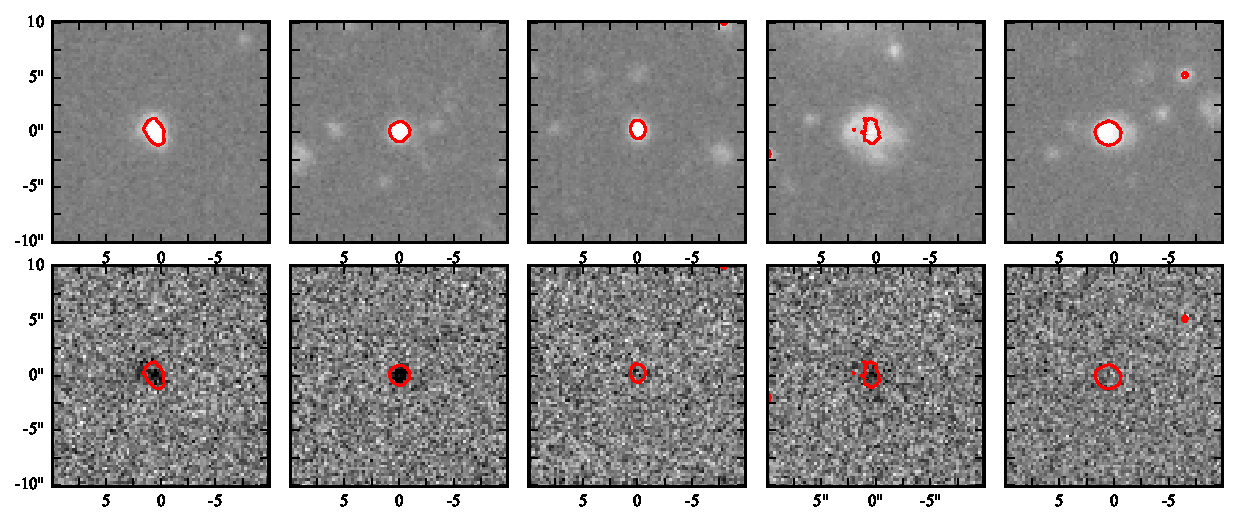
\includegraphics[scale=0.7]{../Figures/stamps.pdf}
\caption{ $10'' \times 10''$ images of each galaxy in our sample. Top row: Continuum flux in ergs/s/cm$^2$/sq.arcsec. Bottom row: Continuum subtracted \ion{Mg}{2} flux.  Absorption can be seen in 4 of 5 galaxies. The red contours represent the outline of the 1$\sigma$ surface brightness limit of continuum flux in the HeII/3000+38 image, defined in Sec. \ref{sec.sb}. The colorbar shows the scaling used for the line emission images.}
\label{fig:stamp_images}
\end{figure*}

\subsection{Surface Brightness Profiles and Limits}\label{sec.sb}

In order to test for the presence of \ion{Mg}{2} emission, we perform aperture photometry on the continuum subtracted images using the python library Photutils. We choose annuli with a radial thickness of 1 pixel or $0.25 ''$, such that, $r_{inner}=r_{outer}-1$ (in pixels). Each annulus is centered on the flux-weighted centroid of the galaxy. By dividing the summed flux in each annulus by the area in arcseconds we produced surface brightness (SB) profiles for each galaxy which are shown in Figure \ref{fig:sb_profiles}. 

The error in this quantity is determined from an RMS image produced by \textbf{SWarp}. We place annuli that are identical to the annuli used to find the SB profiles for each galaxy. To calculate the variance inside each annulus, we sum the RMS pixel values in quadrature, then divide by the area of each annulus. 

To calculate the $1\sigma$ SB limit we follow the recipe found in \cite{Battaia_2015}. We first masked out all the sources, their associated extended halos, and edge noise in both the HEII+47 and HEII/3000+48 images. We then calculate the root-mean-square (rms) of the background in randomly placed 1" apertures. We convert these rms values to SB limits $per$ 1 sq.arcsec aperture. We find that the 1$\sigma$ detection limits per 1 arcsec$^2$ aperture (SB$_1$) are $6.332\times10^{-19}$ ergs sec $^{-1}$ cm$^{-2}$ arcsec$^2$ and $5.808\times10^{-19} $ ergs sec $^{-1}$ cm$^{-2}$ arcsec$^2$ in the HeII/3000 and HeII filters, respectively. With the 1$\sigma$ detection limit, SB$_1$, determined for the continuum+\ion{Mg}{2} (HeII) image, we define an extended annulus to be used to detect any extended \ion{Mg}{2} emission. This extended annulus has an inner radius approximately the size of a unique SB$_1$ isophotal contour for each galaxy. The outer radius will be the inner radius extended by an arbitrary choice of 5 pixels.

The sensitivity required to detect an extended source depends on its size because one can reach lower SB levels by spatially averaging over large apertures. In the ideal case of perfect sky subtraction and continuum subtraction, the 1$\sigma$ SB limit for an extended source is $SB_{1}/\sqrt{A_\text{src}}$, where $A_\text{src}$ is the area in arcsec$^2$ and $SB_{1}$ is the surface brightness limit per 1 arcsec$^2$ aperture. In practice, the actual detection limits are limited by systematics from imperfect subtraction. Therefore, we empirically determine the limits as follows. We mask all the artifacts and sources in the continuum-subtracted images. Next generate randomly sized annuli, place them at random and extract the fluxes, $F_{\text{src}}$, within these annuli. In the ideal case that the sky and continuum are perfectly subtracted, the fluxes, $F_{\text{src}}$, from many random annuli should follow a Gaussian distribution with a width of $\sigma_{\text{src}} \equiv SB_{1}\sqrt{A_\text{src}}$. We find that the actual Gaussian width, $\sigma'_{\text{src}}$ of the distribution is broader than $\sigma_{\text{src}}$. We adopt $F_{\text{limit}} \equiv \sigma'_{\text{src}}$  as the $1 \sigma$ upper limit on the total line flux of extended \ion{Mg}{2} emission. 

\begin{figure}[!ht]
\centering
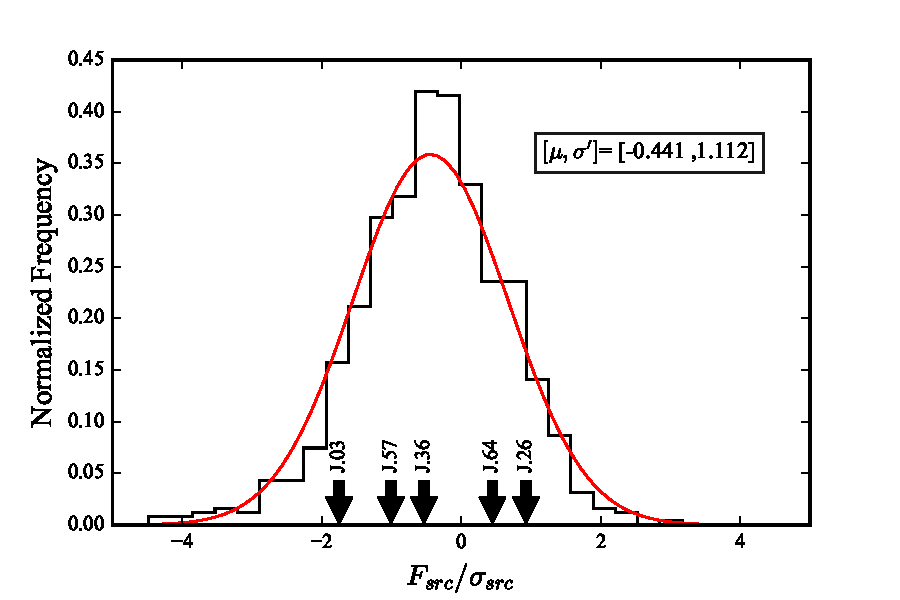
\includegraphics[scale=0.6]{../Figures/hist_sblim.pdf}
\caption{Normalized distribution of $F_{\text{src}}/\sigma_{\text{src}}$ values, for random circular annuli. $F_{\text{src}}$ is the total flux within the largest annulus and $\sigma_{\text{src}}$ is the expected $1\sigma$ flux limit in the ideal case of perfect sky and continuum subtraction, i.e $SB_{1}\sqrt{A_\text{src}}$.}
\label{fig:limits}
\end{figure}

\begin{table}[h]
\centering
%\begin{minipage}{4in}
\caption{Significance of Extracted Flux \label{tab:sb_lims}}  
\begin{tabular}{llll} \hline \hline
Object & F(\ion{Mg}{2})\footnote{\ion{Mg}{2} flux is in $10^{-18}$ ergs sec$^{-1}$ cm$^{-2}$. The value in the parenthesis is the statistical significance with respect to $\sigma_{\text{src}}$ } & Area\footnote{Area of the extended annulus in sq.arcsec} \\  \hline
J033225.26-274524.0 &  2.44(0.92)	& 21 \\
J033232.36-274725.0 &  -1.40(-0.53) & 21 \\
J033230.03-274347.3 &  -5.23(-1.75) & 27 \\
J033229.64-274242.5 &  1.23 (0.44) & 26 \\
J033230.57-274518.2 &  -2.53 (-1.00) & 18 \\ \hline
\end{tabular}
%\end{minipage}
\end{table}

In order to show that our detection limits are reasonable, we create simulated emission with varying intensities to see if we can visually detect any \ion{Mg}{2} emission. The results of this exercise are shown in Figure \ref{fig:sigmas} For each galaxy, we assume a constant surface brightness corresponding to an excess of surface brightness 0, 1, 3, 5, 10 and 20 times the $1\sigma$ SB$_{\text{limit}}$ inside the largest annulus used. Additionally, we assume gaussian noise with a variance equal to 1SB$_{\text{limit}}$. After placing the simulated emission around the galaxy, we subtract the continuum in the same manner as explained in Section \ref{sec.cont_sub}. To test the detectability of measuring extended emission we construct a smoothed $\chi$ image following the technique in \cite{Hennawi2013} and \cite{Battaia_2015}. First, we smooth the continuum-subtracted image:

\begin{equation}
I_{\text{smth}}= \text{CONVOLVE[NB-CONTINUUM]},
\end{equation}
where the CONVOLVE operation indicates convolution of the images with a Gaussian kernel with FWHM=1.5 pixels. Next, we computed the sigma image ($\sigma_{\text{smth}}$) for the smoothed image ($I_{\text{smth}}$) by propagating the noise image of the unsmoothed data:
\begin{equation}
\sigma_{\text{smth}}=\sqrt{\text{CONVOLVE}^2[\sigma^2_{\text{unsmth}}]},
\end{equation}
where the CONVOLVE$^2$ operation indicates the convolution of the noise image with the square of the Gaussian kernel. The smoothed $\chi$ image is defined by
\begin{equation}
\chi_{\text{smth}}=\frac{I_{\text{smth}}}{\sigma_{\text{smth}}}.
\end{equation}
This $\chi_{\text{smth}}$ image aids in recognizing the presence of extended \ion{Mg}{2} emission. 

Figure \ref{fig:sigmas} shows the $\chi_{\text{smth}}$ image for the synthetic \ion{Mg}{2} emission. Galaxies are outlined by a black isophotal contour corresponding to 1SB$_1$ and the simulated emission is contained inside an annulus surrounding the contours. The  $\chi_{\text{smth}}$  images confirm that we should be able to detect extended \ion{Mg}{2} emission down to a conservative level of 5SB$_{\text{limit}}$. Note again that the SB$_{\text{limit}}$ does indeed take into account the systematics from imperfect continuum subtraction. 

\begin{table}[]
\centering
%\begin{minipage}{4.5in}
\caption{Empirically Determined Detection Limits \label{tab:det_lims}}  
\begin{tabular}{llll} \hline \hline
Object & 5SB$_{\text{limit}}$\footnote{Limits are in $10^{-19}$ ergs sec $^{-1}$ cm$^{-2}$ arcsec$^2$} &Area\footnote{Area of the extended annulus in sq.arcsec} \\  \hline
J033225.26-274524.0 &  6.51 & 21 \\
J033232.36-274725.0 & 6.51 & 21 \\
J033230.03-274347.3 & 5.74 & 27 \\
J033229.64-274242.5 & 6.22  & 26 \\
J033230.57-274518.2 & 6.81 & 18 \\ \hline
\end{tabular}
%\end{minipage}
\end{table}

\begin{figure*}[p]
\centering
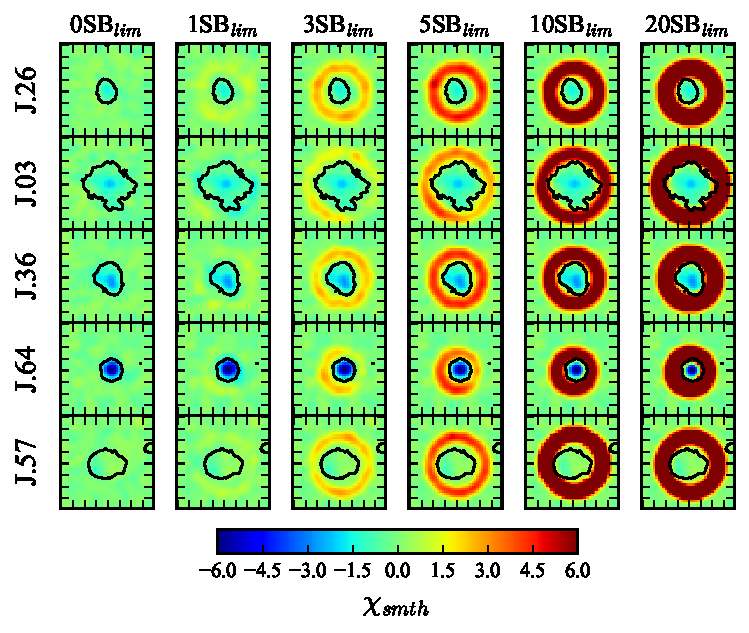
\includegraphics[scale=1.2]{../Figures/sigmas.pdf}
\caption{Postage stamp $\chi_{\text{smth}}$ images of the 5 galaxies in our sample. Every galaxy is placed in the same row in each column. The columns show simulated emission, with levels of 0, 1, 3, 5, 10, and 20 times SB$_{lim}$.  Each postage stamp has a size of $5'' \times 5''$ (corresponding to $35$ kpc $\times$ $35$ kpc at $z\sim 0.70$). Each stamp shows the galaxy along with the same isophotal contour used in previous figures. Comparing the $0$SB$_{\text{limit}}$ column with the continuum-subtracted images in Figure \ref{fig:stamp_images} suggests that we did not detect any \ion{Mg}{2}\ emission.}
\label{fig:sigmas}
\end{figure*}


\subsection{Equivalent Widths}\label{subsec.ew}
Here we derive an expression to calculate the equivalent width (EW) of any absorption or emission features observed in our narrow-band imaging. Starting from the expression for EW used in the context of spectroscopy,
\begin{equation}
EW=\int (1-\frac{f_{line}}{f_{cont}})d\lambda
\label{eq:specEW}
\end{equation}
we begin by dividing Eq \ref{eq:subtraction} by the flux density of the continuum and the FWHM of the on-line filter,
\begin{equation}
\frac{F_{line}}{f_{cont}\Delta \lambda_{MgII}}=\frac{F_{MgII}}{f_{cont}\Delta \lambda_{MgII}}- 1.
\end{equation}
Next, we rearrange the above expression such that we produce the argument of the integrand in Eq. \ref{eq:specEW} on the RHS,
\begin{equation}
-\frac{F_{line}}{f_{cont}\Delta \lambda_{MgII}}=1-\frac{f_{MgII}}{f_{cont}}.
\end{equation}
We then approximate the integration in Eq. \ref{eq:specEW} by multiplying the integrand above by the FWHM of the on-line filter $d\lambda=\Delta \lambda_{MgII},$
\begin{equation}
-\frac{F_{line}}{f_{cont}}=(1-\frac{f_{MgII}}{f_{cont}})\Delta \lambda_{MgII};
\end{equation}
such that
\begin{equation}
EW=-\frac{F_{line}}{f_{cont}}.
\end{equation}

Using the above equation along with the continuum and continuum-subtracted images, we produce images of the EWs. The EW images are displayed in Figures \ref{fig:ew11}, \ref{fig:ew22}, \ref{fig:ew33}, \ref{fig:ew44}, \ref{fig:ew55}, and show only the EWs within the 1$\sigma$ SB$_1$ contours of the corresponding \ion{Mg}{2} images (prior to continuum subtraction). 

To compare our map of EWs to the values measured from the Keck/LRIS spectra, we place 0.9 arcsec wide apertures on top of each galaxy. The width and angle of the apertures replicate the orientation of the slits used to obtain the spectra. Next, we determine which pixels lie outside the 1$\sigma$ SB$_1$ contours and set those to zero. Outside this contour, the EWs become poorly constrained due to the lack of S/N in the continuum. We then apply a S/N $= 1.5$ cut to the continuum image and create a histogram to show the distribution of EWs as shown in Figures \ref{fig:ew1} through \ref{fig:ew5}. Having removed EWs with low-S/N continuum values from our images, we compute the mean equivalent width inside the Keck/LRIS apertures. These values are summarized in Table \ref{tab:abs_props}.
 
In order to get information on the morphology of the \ion{Mg}{2}, we determine the distance of each pixel from the center of each galaxy in kiloparsecs. We plot the EWs over this projected distance for each galaxy in Figures \ref{fig:ew1} through \ref{fig:ew55}. Although some of the plots suggest a slight upward trend in the values of the EW at increasingly large radii, we cannot be confident in this trend because of large scatter. To better visualize the data and test the significance of the trend, we bin the data radially. For example, in Figure \ref{fig:ew44}, the EW from absorption extends out to $\sim$ 25 kpc. The EWs are binned in 5 kpc increments. We calculate the mean and scatter of the EWs in each bin and show these values in Figure \ref{fig:ew_comb}.   


\section{Discussion}\label{sec.results}
In this chapter we present the results from the continuum-subtraction of the off-line continuum filter to that of the on-line emission filter. 

\subsection{Limits on MgII emission}

We do not detect any significant amount of \ion{Mg}{2} emission in any of our sampled galaxies. The $\chi_{\text{smth}}$ images shown in Figure \ref{fig:sigmas} confirm this. A comparison of the simulated emission with the $\chi_{\text{smth}}$ image of the original stamps, shown in the first column, similarly suggests that we do not detect any extended \ion{Mg}{2} emission. We thus place conservative $5\sigma$ upper limits on \ion{Mg}{2} emission for each galaxy in the sample, summarized in Table \ref{tab:det_lims}. The most sensitive detection limit using the largest area is SB(\ion{Mg}{2}) = 5.74 $\times$ $10^{-19}$ ergs sec $^{-1}$ cm$^{-2}$ arcsec$^2$, computed for the galaxy J033230.03. Our least sensitive detection limit is SB(\ion{Mg}{2}) = 6.81 $\times$ $10^{-19}$ ergs sec $^{-1}$ cm$^{-2}$ arcsec$^2$, computed for the galaxy J033230.57.

\subsection{Previous Detections of extended \ion{Mg}{2} emission}
Previous constraints on the brightness of scattered \ion{Mg}{2} emission were reported by \cite{Rubin_2011}. In this work the authors studied emission from the starburst galaxy TKRS 4389 at $z = 0.69$ with a star formation rate of $49.8\msunperyr$. This emission was detected in a 2-dimensional KECK/LRIS spectrum, with flux from the emission reaching $8.0 \pm 0.4$ and $4.4 \pm 0.4$ $\times10^{-18}$ ergs sec$^{-1}$ cm$^{-2}$ at  $\lambda _{2796}$ and $4.0 \pm 0.3$ and $2.5 \pm 0.4$ $\times10^{-18}$ ergs sec$^{-1}$ cm$^{-2}$ at $\lambda_{2803}$ in two independent locations spatially offset from the galaxy continuum. The flux from the emission can be converted into two surface brightness values by taking the average of the flux measured at each location and each transition, and dividing by a 1 sq.arcsec aperture. 

Figure \ref{fig:detection_lim} shows a plot of the 5$\sigma$ detection limits determined for each galaxy in our sample as well as the SB calculated for the galaxy TKRS 4389. The figure suggests that we should be able to detect scattered \ion{Mg}{2} emission with strengths similar to that detected in TKRS 4389. Given if  additional detections of extended \ion{Mg}{2} emission are made, it could be possible that there exists the possibility of a relationship between SB and star-formation rate, as the study by \cite{Erb2012} discuss that emission strength is stronger in high mass galaxies. This could be one explanation as to why we did not detect any extended \ion{Mg}{2} emission Further studies need to be pursued to add additional points to Figure \ref{fig:detection_lim}.

\subsection{Geometry of re-emitted photons}
In idealized wind models of cool gas outflows, discussed in \cite{Prochaska_2011}, strong \ion{Mg}{2} emission is predicted to be generated along with ubiquitous blueshifted absorption of \ion{Mg}{2}. For isotropic and dust-free scenarios, this absorption and emission is simply produced by the conservation of photons, as any absorbed continuum photon is eventually re-emitted in emission. Because of this photon exchange the total equivalent width of both the absorption and emission features is equal to zero.
Assuming that our galaxies host an isotropic and dust-free wind, we wish to determine how much emission is predicted to be missing from our imaging, and how the SB of this missing emission compares to our detection limits, for different distributions of emission. 

To find the amount of missing emission, we first need to calculate how much continuum has been absorbed by \ion{Mg}{2}. Using our Keck/LRIS spectra, we find the average value of the continuum near the \ion{Mg}{2} doublet and multiply this value by the EW of the doublet. Although we know how much emission is missing, we do not know how this emission is distributed outside the galaxy. As a conservative estimate of the SB, we distribute the missing emission uniformly inside multiple and increasingly sized annuli. These annuli are fixed to have an inner radius equal to the galaxy's isophotal radius and an increasing outer radius.  Additionally, since our SB limits are dependent on the size of the aperture used, we calculate the SB limits inside each of the aforementioned annuli. Figure \ref{fig.emission} shows how the SB of emission varies with the spatial extent of the annulus, as well as how the SB compares with our detection limits.. 

Excluding the galaxy J033230.03, the SB of this missing emission lie above our detection limits. This result shows that these galaxies do not host an isotropic dust-free wind.


\begin{figure}[!htb]
\centering
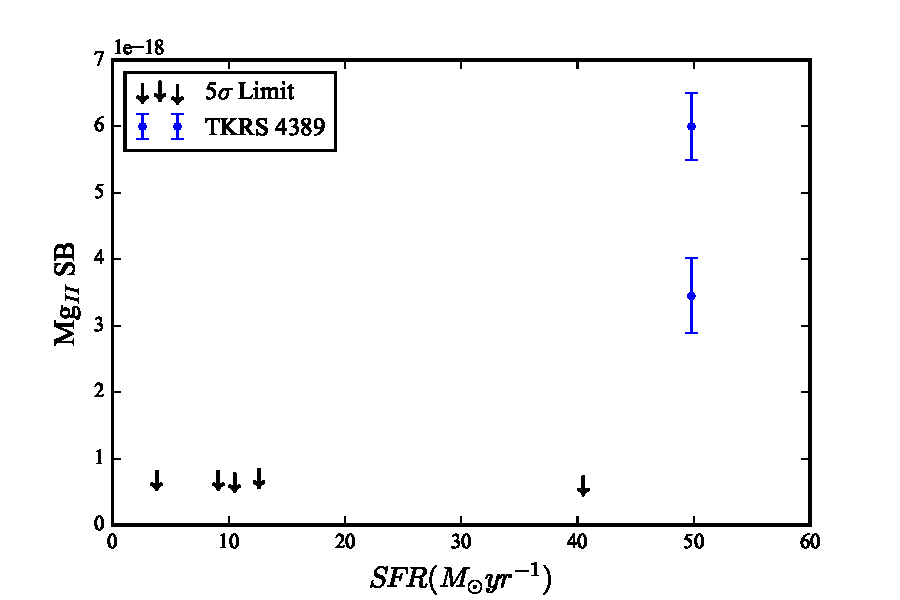
\includegraphics[scale=0.6]{../Figures/limits.pdf}
\caption{Comparison of our detection limits to the measured extended emission of TKRS 4389. Our imaging is sufficiently sensitive to detect extended emission at similar strengths to the extended emission measured for TKRS 4389.}
\label{fig:detection_lim}
\end{figure}

\subsection{Spatially Resolved Maps of \ion{Mg}{2} Absorption}
In this section we discuss the details of the absorption detected in our images and compare our measurements to those obtained in the Keck/LRIS spectra of each galaxy.. 

\subsubsection{\ion{Mg}{2}\ absorption in surface brightness profiles}
Although we do not detect any extended \ion{Mg}{2} emission, we do observe a decrement of flux in the SB profiles of 4 out of 5 galaxies in our sample. 

\subsubsection{J033225.26} 
Figure \ref{fig:sb_profiles} shows the SB profile for J033225.26. We report that the maximum decrement in the SB profile due to absorption is strongest at the center of the galaxy. The SB measured in the center aperture is -5.39 $\pm$ 0.128 $\times10^{-18}$ erg s$^{-1}$ cm$^{-2}$ per sq.arcsec. The absorption in the profile decreases radially outward and is detected out to the largest distance sampled, $\sim 18$ kpc, away from the center of the galaxy.

\subsubsection{J033231.36} 
Figure \ref{fig:sb_profiles} shows the SB profile for J033231.36. We report that the maximum decrement in the SB profile due to absorption is strongest at the center of the galaxy. The SB measured in the center aperture is -5.64 $\pm$ 0.121 $\times10^{-18}$ erg s$^{-1}$ cm$^{-2}$ per sq.arcsec. The absorption in the profile decreases radially outward and is detected out to the largest distance sampled, $\sim 18$ kpc, away from the center of the galaxy.

\subsubsection{J033230.03} 
Figure \ref{fig:sb_profiles} shows the SB profile for J033230.03. We report that the maximum decrement in the SB profile due to absorption is strongest at the center of the galaxy. The SB measured in the center aperture is -4.41 $\pm$ 0.622 $10^{-18}$ erg s$^{-1}$ cm$^{-2}$ per sq.arcsec. The absorption in the profile decreases radially outward and out to the largest distance sampled, $\sim 25$ kpc, away from the center of the galaxy.

\subsubsection{J033229.64} 
Figure \ref{fig:sb_profiles} shows the SB profile for J033229.64. We report that the maximum decrement in the SB profile due to absorption is strongest at the center of the galaxy. The SB measured in the center aperture is -18.2 $\pm$ 0.127 $\times10^{-18}$ erg s$^{-1}$ cm$^{-2}$ per sq.arcsec. The absorption in the profile decreases radially outward and is detected out to the largest distance sampled, $\sim 14$ kpc, away from the center of the galaxy.

\subsubsection{J033230.57} 
Figure \ref{fig:sb_profiles} shows the SB profile for J033230.57. The absorption decrement is strongest at the center of the galaxy with a SB value of -1.25 $\pm$ 1.15 $10^{-18}$ erg s$^{-1}$ cm$^{-2}$ per sq.arcsec. However, the measured SB of this decrement including error is consistent with measuring zero absorption. The measurement of zero absorption for J033230.57 was expected. Figure \ref{fig:spec_images} shows the KECK/LRIS spectrum of J033230.57 and the transmission curves of the filters HeII+47 and HeII/3000+48. The \ion{Mg}{2} transitions of the galaxy are equally sampled by both of our filters. Simply put, each image of J033230.57 contains equal amounts of continuum and \ion{Mg}{2}. When we subtract the continuum image from the \ion{Mg}{2} image we are effectively canceling out the \ion{Mg}{2} absorption as well. This measurement can stand as a test of the quality of our continuum subtraction. \\

The surface brightness profiles presented in Figures \ref{fig:sb_profiles} do not exhibit any signs of extended \ion{Mg}{2} emission. \\

\subsection{Morphology of MgII Absorption}

Figures \ref{fig:ew1} through \ref{fig:ew5} show the EW images, distributions and radial projections of \ion{Mg}{2} EWs. We have zeroed out any EWs that lie outside the SB$_1$ contours for each galaxy. We imposed a signal-to-noise cut, only including EWs where the continuum flux S/N greater than $|1.5|$. The mean EW is computed for all pixels inside each Keck/LRIS aperture, defined in Sec. \ref{subsec.ew}, and are summarized in Table \ref{tab:abs_props}. Comparing our measured EWs with those measured from the spectra, we find good agreement to within 1$\sigma$ or 2$\sigma$ for most of the galaxies except and J033230.57.

In the case of J033230.57 we can easily understand why the EW measured is not in agreement with the spectra EW. Figure \ref{fig:sb_profiles}  shows the SB profile coverage of J033230.57, in this galaxy's profile we do not detect any significant decrements due to absorption. This is due to the fact that our two filters cover the \ion{Mg}{2} doublet equally, see Figure  \ref{fig:spec_images}. Any signal of absorption in the EW images arise from noise. Figure \ref{fig:ew5} shows the radial projection of the EWs measure for this galaxy which are centered around zero.

To get a better sense of how the EW of \ion{Mg}{2} absorption changes with radius as well as account for any effects due to seeing, $\sim 7 kpc$, we bin the EWs in radial bins with 5, 4 or 3 kpc widths as shown in Figures \label{fig:ew1} through \label{fig:ew5}. A majority of the galaxies appear to show large scatter in the EWs out to larger radii. To better understand the significance of these trends, we construct a plot that compiles the mean EWs for all the galaxies, shown in Figure \ref{fig:ew_comb}. To take into account the varying size of the galaxies, we normalize the distances by the approximate radius of the SB$_1$ contour for each galaxy. 

Upon inspection of Figure \ref{fig:ew_comb}, we see that all the galaxies exhibit a constant mean EW inside our 1SB$_1$ isophotal radius.

\section{CONCLUSION AND FUTURE WORK}
We presented the results from a narrowband imaging search for \ion{Mg}{2} emission in a sample of star-forming galaxies at a redshift of $z \sim 0.70$.  Although we were unable to detect any measurable amount of \ion{Mg}{2} emission, we are able to report a conservative $5\sigma$ detection limit of  SB(\ion{Mg}{2}) = 5.74 $\times 10^{-19}$ ergs sec $^{-1}$ cm$^{-2}$ arcsec$^2$. We detected a significant amount of \ion{Mg}{2} absorption in a total of 4 galaxies out of our 5 galaxy sample. Furthermore, our imaging allows us to generate spatially-resolved maps of \ion{Mg}{2} absorption in a distant galaxy sample for the first time. This absorption covered the center of the galaxies out to the SB$_1$ continuum + \ion{Mg}{2} isophotal radius, at approximately $\sim 22$ kpc, suggesting that the absorbing gas fully covers the stellar disks out to this distance. The measured EWs measured in these maps are in broad agreement with measured EWs using Keck/LRIS integrated slit spectroscopy. Additionally, our radial projections of the mean EW for our sample galaxies suggest that the EWs due to \ion{Mg}{2} are approximately constant out towards the edges of the galaxies. Finally, we compared our detection limits with estimated SB \ion{Mg}{2} emission, based on the radiative transfer models of \cite{Prochaska_2011}. For an isotropic dust-free wind, \ion{Mg}{2} is predicted to be generate alongside ubiquitous \ion{Mg}{2} absorption. Our detection limits are suitable to detect the estimated SB \ion{Mg}{2} emission and since we do not detect the excess emission, the  isotropic morphology of a wind is ruled out in our galaxy sample.

In the future, we hope to observe these galaxies using an Integral Field spectrograph (IFU). IFUs take the signal from an individual pixel and feeds it into a spectrograph. The spectrograph then generates a spectrum for that pixel, allowing us to view the flux at specific transitions. IFUs cover large 2D fields of view, contrary to single point 1D spectroscopy or the slice of 2D longslit spectroscopy, makes them exceptionally useful in resolving the spectrum of a target for multiple sightlines. Thus, IFUs are useful in detecting the gas of extended objects, such as galaxies. Because IFUs would allow us to observe the spectrum of a galaxy's extended region, we will be able to compare our EW maps, as well as EW radial projections, with higher resolution observations. 

Based on the radial extent and strength of our measured \ion{Mg}{2} absorption, the \ion{Mg}{2} is optically thick. However, we need to compare our measured absorption strength and radial extent with radiative transfer models. In the radiative transfer models of \cite{Prochaska_2011}, scattered emission is predicted for an isotropic, optically thick,and dust free wind with density that decreases as an inverse square law, however galaxies are not spherically symmetric and sources driving the wind may not be distributed spherically. Allowing for a bi-conical anisotropic wind, \cite{Prochaska_2011} state that the scattered \ion{Mg}{2} emission will become suppressed compared to the strengths an isotropic wind. Future observations of our galaxies in IFUs could perhaps shed light on this alternate scenario.



\begin{figure*}
\centering
\gridline{\fig{../Figures/J033225_26.pdf}{0.5\textwidth}{(J033225.26)}
          \fig{../Figures/J033231_36.pdf}{0.5\textwidth}{(J033231.36)}}
\gridline{\fig{../Figures/J033230_03.pdf}{0.5\textwidth}{(J033230.03)}
          \fig{../Figures/J033230_64.pdf}{0.5\textwidth}{(J033230.64)}}
           \fig{../Figures/J033230_57.pdf}{0.5\textwidth}{(J033230.57)}
\caption{SB profile for our sample galaxies. (Top) Continuum SB (black) measured for the galaxy in the continuum image. Mg II + continuum SB (green) measured for the galaxy in the pre-continuum subtracted image. Mg II line SB (blue) measured for the galaxy in the continuum subtracted line emission image.The profile exhibits SB decrements from \ion{Mg}{2} absorption. Photometry was performed in circular annuli. (Bottom) The vertical hashes in the bottom show the inner and outer radius of each annulus in kpc. Distance from the center of the galaxy (x-axis) is computed using the average value of each annulus inner and outer radii of each annuli.}
\label{fig:sb_profiles}
\end{figure*}


 \begin{figure*}[]
\centering
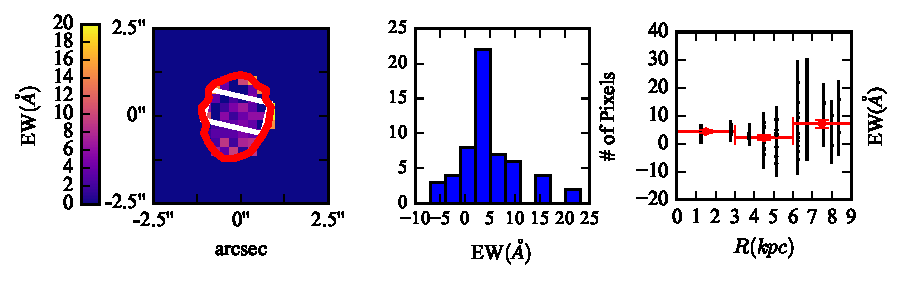
\includegraphics[scale=0.9]{../Figures/J26EW.pdf}
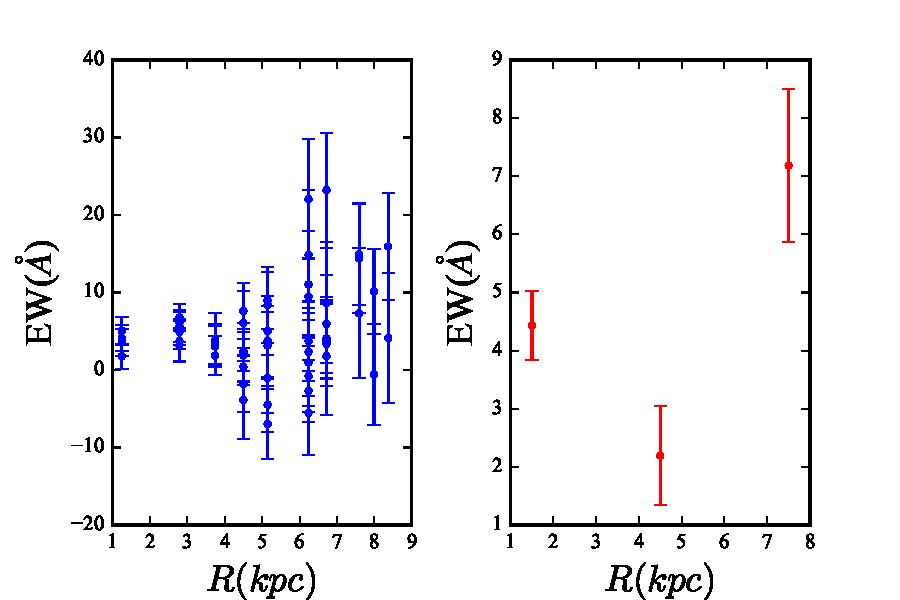
\includegraphics[scale=0.9]{../Figures/J26EW_2.pdf}
\caption{Equivalent width images, distribution and radial projection for J033225.26. (Top Left) image of the \ion{Mg}{2} equivalent widths inside the red 1SB$_1$ contour. The white contour represents the $0.9''$ wide  slit used to measure the equivalent width of absorption in the Keck/LRIS spectra.  (Top Right) Distribution of absorption pixels with continuum flux S/N greater than 1.5 inside the slit aperture. (Bottom Left) The EWs of absorption vs projected distance from center. (Bottom Right) Binned EW measurements. Each point represents the mean EW measured in 3 kpc wide bins.}
\label{fig:ew11}
\end{figure*}

\begin{figure*}[]
\centering
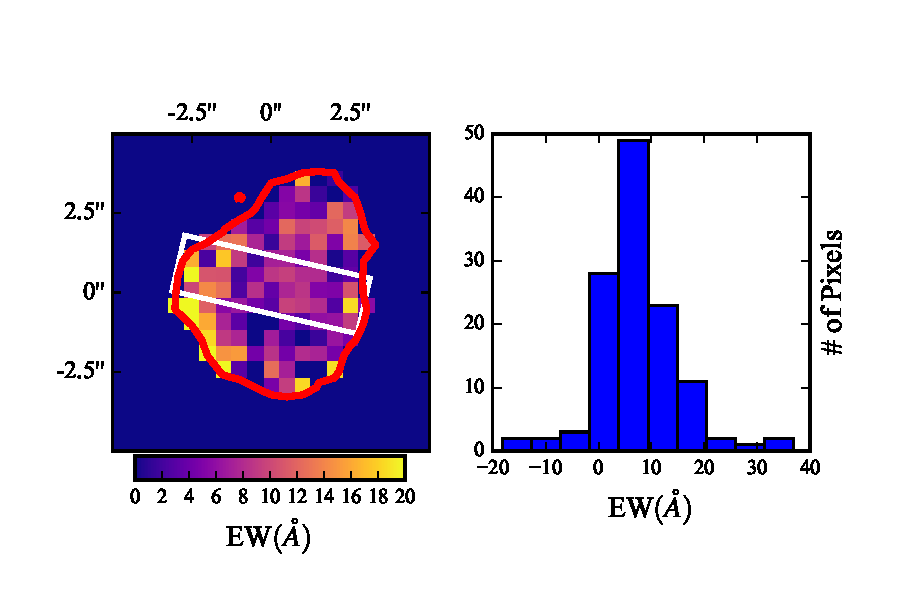
\includegraphics[scale=0.9]{../Figures/J36EW.pdf}
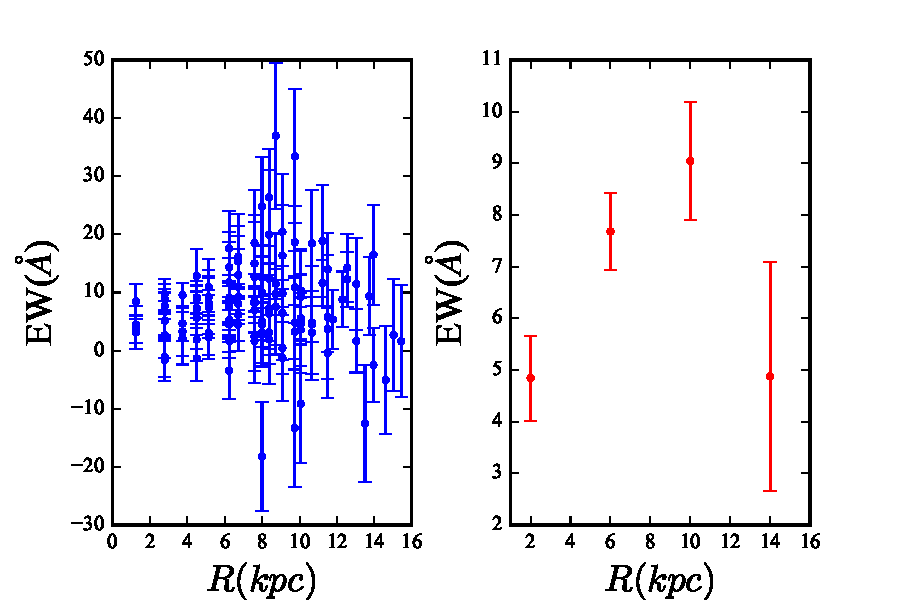
\includegraphics[scale=0.9]{../Figures/J36EW_2.pdf}
\caption{Equivalent width images, distribution and radial projection for J033231.36. (Top Left) image of the \ion{Mg}{2} equivalent widths inside the red 1SB$_1$ contour. The white contour represents the $0.9''$ wide  slit used to measure the equivalent width of absorption in the Keck/LRIS spectra.  (Top Right) Distribution of absorption pixels with continuum flux S/N greater than 1.5 inside the slit aperture. (Bottom Left) The EWs of absorption vs projected distance from center. (Bottom Right) Binned EW measurements. Each point represents the mean EW measured in 4 kpc wide bins.}
\label{fig:ew22}
\end{figure*}

\begin{figure*}[]
\centering
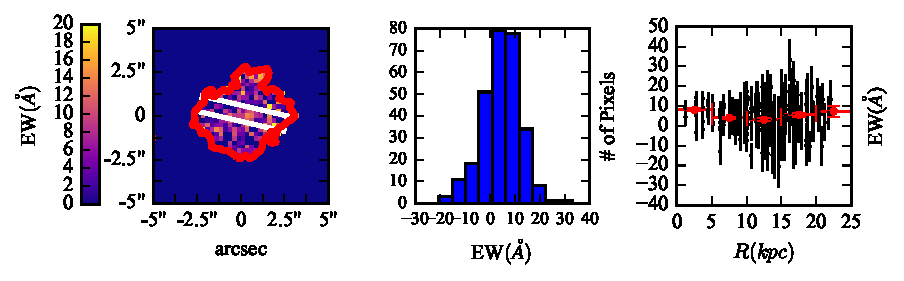
\includegraphics[scale=0.9]{../Figures/J03EW.pdf}
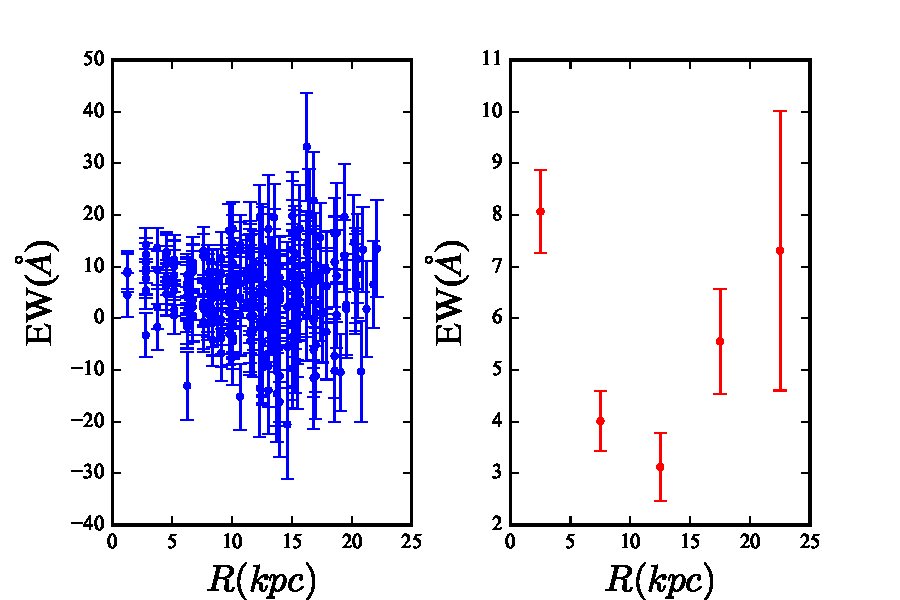
\includegraphics[scale=0.9]{../Figures/J03EW_2.pdf}
\caption{Equivalent width images, distribution and radial projection for J033230.03. (Top Left) Stamp of the equivalent widths (EWs) inside the red 1SB$_1$ contour. The white contour represents the $0.9''$ aperture slit used to measure the equivalent width of absorption in the Keck/LRIS spectra. (Top Right) Distribution of absorption pixels with continuum flux S/N greater than 1.5 inside the slit aperture. (Bottom Left) The EWs of absorption projected in distance from center. (Bottom Right) Binned EW measurements. Each point represents the mean EW measured in 5 kpc increment bins. }
\label{fig:ew33}
\end{figure*}

\begin{figure*}[]
\centering
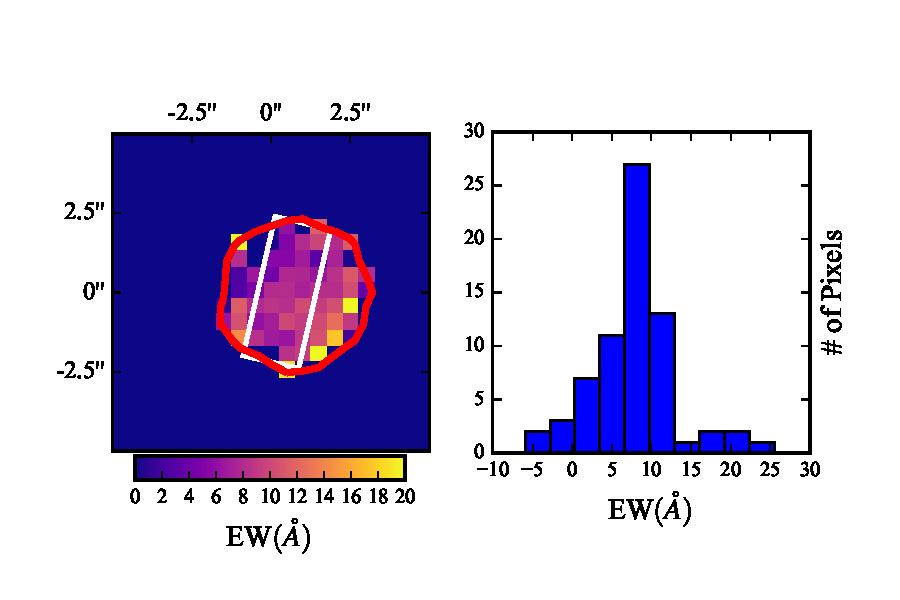
\includegraphics[scale=0.9]{../Figures/J64EW.pdf}
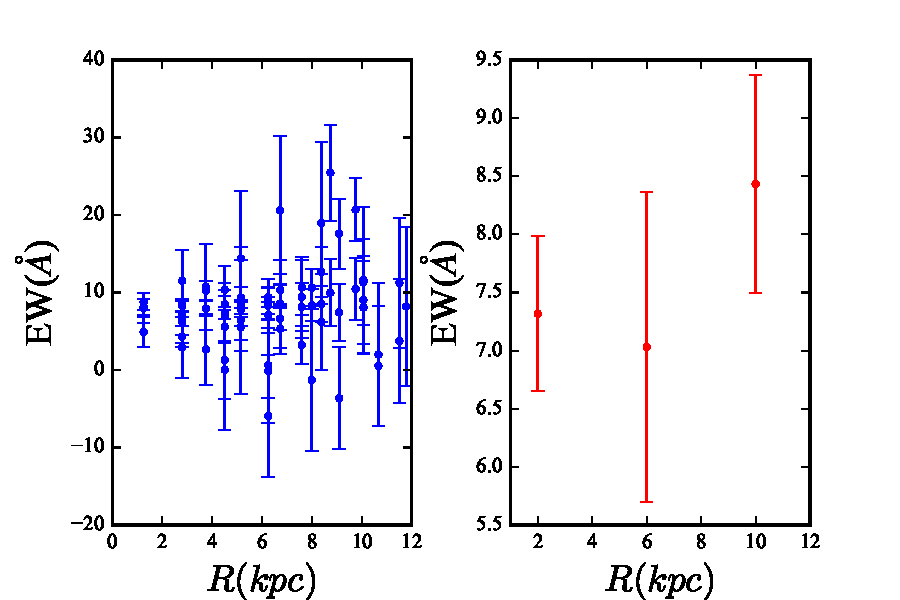
\includegraphics[scale=0.9]{../Figures/J64EW_2.pdf}
\caption{ Equivalent width images, distribution and radial projection for J033229.64. (Top Left) Stamp of the equivalent widths (EWs) inside the red 1SB$_1$ contour. The white contour represents the $0.9''$ aperture slit used to measure the equivalent width of absorption in the Keck/LRIS spectra. (Top Right) Distribution of absorption pixels with continuum flux S/N greater than 1.5 inside the slit aperture. (Bottom Left) The EWs of absorption projected in distance from center. (Bottom Right) Binned EW measurements. Each point represents the mean EW measured in 4 kpc wide bins.}
\label{fig:ew44}
\end{figure*}

\begin{figure*}[]
\centering
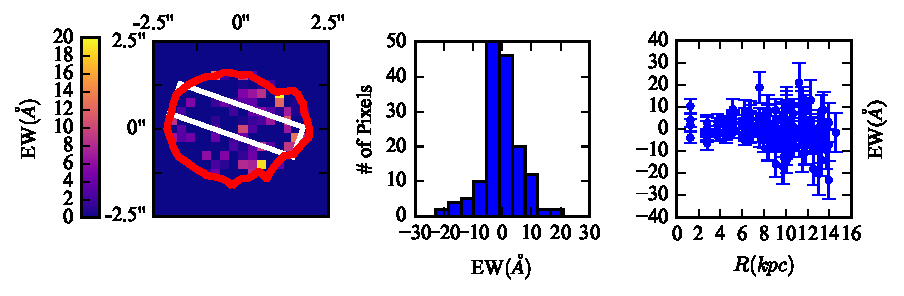
\includegraphics[scale=0.9]{../Figures/J57EW.pdf}
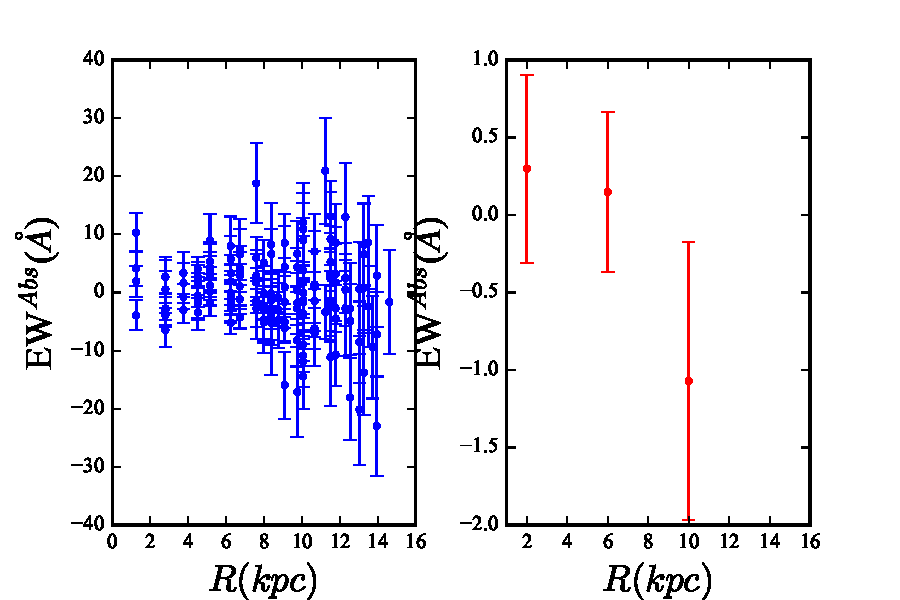
\includegraphics[scale=0.9]{../Figures/J57EW_2.pdf}
\caption{Equivalent width images, distribution and radial projection for J033230.57. (Top Left) Stamp of the equivalent widths (EWs) inside the red 1SB$_1$ contour. The white contour represents the $0.9''$ aperture slit used to measure the equivalent width of absorption in the Keck/LRIS spectra. (Top Right) Distribution of absorption pixels with continuum flux S/N greater than 1.5 inside the slit aperture. (Bottom Left) The EWs of absorption projected in distance from center. (Bottom Right) Binned EW measurements. Each point represents the mean EW measured in 4 kpc wide bins.}
\label{fig:ew55}
\end{figure*}

\begin{figure*}[!htb]
\centering
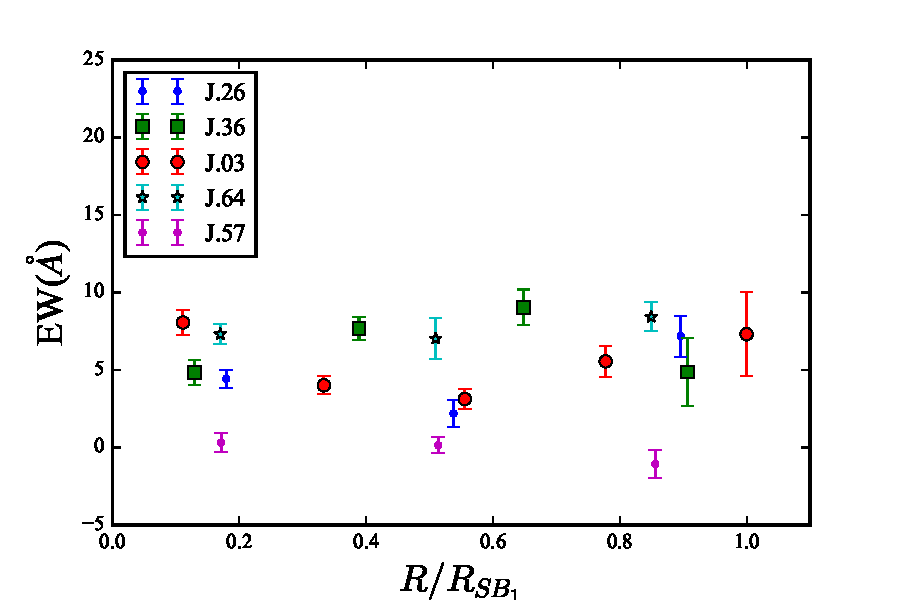
\includegraphics[scale=0.9]{../Figures/ew_comb.pdf}
\caption{Normalized radial profile of the mean EW of \ion{Mg}{2} absorption for all galaxies. Measurements for the mean EW binned in radial increments compiled to test the significance of any trends found in the individual galaxy profiles. There is significant scatter relative to the error bars at extended distances.}
\label{fig:ew_comb}
\end{figure*}

\begin{table*}[]
\centering
\caption{Properties of \ion{Mg}{2}\ Absorption\label{tab:abs_props}}  
\begin{tabular}{llllll} \hline \hline
Object & Max(SB$_{abs}$)\footnote{SB Values are in units of $10^{-18}$ ergs sec $^{-1}$ cm$^{-2}$ arcsec$^2$} & $R_{\text{SB}_1}(kpc)$ &\ \ \ EW($\AA$)\footnote{ Measured from EW images} & EW($\AA$)\footnote{Measured from Keck/LRIS spectra}  \\  \hline
J033225.26-274524.0 &  $-5.39 \pm 1.28 $ & 8 &     $\ \ \ 3.511 \pm 0.795$ & $7.539 \pm 0.354 $\\
J033232.36-274725.0 &  $-5.64 \pm 0.121 $ & 15 & $\ \ \ 7.694 \pm 1.016$ & $5.835 \pm 0.493$\\
J033230.03-274347.3 &  $-4.41 \pm 0.622 $ & 21 & $\ \ \ 5.388 \pm 0.712$ & $12.79 \pm 1.710$\\
J033229.64-274242.5 &  $-18.2 \pm 0.127 $ & 10 & $\ \ \ 7.546 \pm 0.660$ & $13.24 \pm 0.263$\\
J033230.57-274518.2 &  $-1.25 \pm 1.15   $ & 11& -$0.6532 \pm 0.589$ & $6.106 \pm 0.370$\\ \hline
\end{tabular}
\end{table*}
 
\begin{figure*}
\centering
\gridline{\fig{../Figures/geo_J26.pdf}{0.5\textwidth}{(J033225.26)}
          \fig{../Figures/geo_J36.pdf}{0.5\textwidth}{(J033231.36)}}
\gridline{\fig{../Figures/geo_J03.pdf}{0.5\textwidth}{(J033230.03)}
          \fig{../Figures/geo_J64.pdf}{0.5\textwidth}{(J033230.64)}}
\caption{ Estimated SB profile of \ion{Mg}{2} emission. The square points are SB of missing \ion{Mg}{2} emission uniformly distributed inside an annulus. The solid line shows the value of the SB detection limits. The dashed vertical and horizontal lines represent outer radius of }
\label{fig.emission}
\end{figure*}


\newpage
\bibliography{references2017}






\end{document}